% Setup
\documentclass[]{hdsr}
\graphicspath{{graphics/}}

\begin{document}
\newgeometry{bottom=1.0in}
\volumeheader{FE}{690}{Machine Learning in Finance}

% Title
\begin{center}
  \title{Latent Dirichlet Allocation on SOMETHING to Extract a Trading Signal}
  \maketitle

% Authors
Author: Theo Dimitrasopoulos\upstairs{\affilone*}, Advisor: Zachary Feinstein\upstairs{\affilone**}\\
{\small \upstairs{\affilone}Department of Financial Engineering; Babbio School of Business}

% Emails  
\emails{
\upstairs{*}\textit{tdimitr1@stevens.edu,}
\upstairs{**}\textit{zfeinste@stevens.edu}
}
\vspace{0.15in}

% Abstract
\begin{abstract}
This paper focuses on Regime Detection in historical markets. It utilizes a Hidden Markov Model (hereinafter referred to as HMM) and Support Vector Machine (hereinafter referred to as SVM) to detect regimes in the iShares MSCI EAFE ETF adjusted close price time series from 2000 to today (chosen mainly due to its greater exposure to overseas mid- and large-cap companies), in order to enable the accurate prediction of the 24-hour trend of a market-on-open order in a domestic exchange. We observe that the HMM accurately predicts regimes in the historical time series very effectively and in relatively short timespans. It is also shown that the classified data after an unsupervised SVM clustering is further enhanced and the regimes further refined. The accuracy is the SVM clusters is heavily influenced by the parameter ν and γ of the Radial Basis kernel Function, as demonstrated is a series of experiments where each of the parameters is altered. The results of the classification can be used to develop a trading strategy for a market-on-open order that is informed by historical market fluctuations.
\end{abstract}
\end{center}

\vspace*{0.15in}
\small
Keywords: {Bear Market, Bull Market, Classification, Clustering, EFA, ETF, Hidden Markov Model, Historical Markets, iShares MSCI, Kernel Function, Machine Learning, Markov States, Regime Detection, Support Vector Machine, Radial Basis Function, Time Series, VIX}


% These commands need to appear at the point where you want the first page to end.
\restoregeometry
\newgeometry{bottom=1.0in}

\section{Introduction}
\label{sec1}
The accurate prediction of stock market movements is one of the hallmarks of quantitative finance and algorithmic trading. However, describing stock market behavior in the past is also of great importance and enables prediction in the first place. The focus of this paper is the accurate identification of regimes in historical markets and their classification as either bull or bear markets. To achieve this, two of the most widely used classification algorithms are deployed to analyze the resulting models for the regime detection task. As such, the longer training times of SVM's otherwise robust kernel methodologies on non-linear discriminants along with the speed and efficiency of a HMM provide a close inspection of the main tools for feature detection and market classification. The tools presented in this work respond to the inherent need and high value of good forecasting models for market-on-open orders, as well as the barriers to creating them. In addition to the innate difficulty in predicting market direction, the fair and transparent procedures set forth by the various American and international exchanges (e.g. NASDAQ's opening cross auction procedure) add to the intractability of the problem.\\
The motivation behind the choice of this particular ETF (iShares MSCI EAFE ETF, or EFA by its ticker) simply lies in the time difference between the US and international markets; Since the aim of the tool is to accurately inform a market-on-open order in a US exchange, the closest proxy to after-hours market data is foreign developments and trading activity overseas. In other words, domestic markets close at 4pm, but international markets are active before the next day's opening and dramatically influence the levels and state of that market.


\section{Hidden Markov Models}
\label{sec2}
HMM’s are designed to augment Markov chains, and will thus be briefly described in this section. A Markov chain describes the probabilities of sequences of random variables, or states. A stochastic process that possesses the Markov property assumes that in order to predict the future, all that matters is the current state of the system (as opposed to a process that possesses the martingale property), and not the full history[1].
\\
Formally,
\begin{equation}
-\frac{\hbar^2}{2m} \frac{d^2 \psi}{dx^2} + V\psi = E\psi\\
\end{equation}

In addition, the probability of a series of output observations yi depends solely on the state that created the series of observations xi [3].
\\
As such, (X,Y) is a HMM if X is a Markov chain (as defined above) and,

\begin{equation}
-\frac{\hbar^2}{2m} \frac{d^2 \psi}{dx^2} + V\psi = E\psi\\
\end{equation}

Similar to Xt, Yt does not depend on the history of X and is observable at time t [1].\\
Formally,

\begin{equation}
-\frac{\hbar^2}{2m} \frac{d^2 \psi}{dx^2} + V\psi = E\psi\\
\end{equation}

In summary, HMM’s aim to solve three fundamental problems [1]:\\
1.	Likelihood: Given a HMM and an observation sequence, what is the likelihood of observing an unclassified sequence?\\
2.	Decoding: Given a HMM and an observation sequence, what is the ideal sequence of the Markov chain X?\\
3.	Learning: Given an observation sequence and potential hidden states in a Borel set, what are the best parameters for the HMM?\\

\section{Support Vector Machines}
\label{sec3}
In the realm of novelty and outlier detection, the original work of Vapnik and Chevronenkis in 1963 set the ground for one of the most widely used and effective tools for the task: the SVM algorithm. In this work, the One-Class SVM with a Radial Basis Function kernel is used.\\
For any SVM, a quadratic programming problem that separates support vectors from the training data lies at the core [2]. The QP solver scales between O(Nfeatures*nsamples2)  and O(nfeatures*nsamples3), thus generating the long runtimes that SVM’s are known for. The Radial Basis kernel function is the following,

\begin{equation}
-\frac{\hbar^2}{2m} \frac{d^2 \psi}{dx^2} + V\psi = E\psi\\
\end{equation}

The parameter γ>0 defines the influence of each training sample i.e. a smaller γ affects other samples less, as they can be farther away [2]. A second parameter ν=0.1 is defined in the model, which approximates the fraction of training errors and support vectors, and is set at 0.1, since the scikit-learn documentation section that tests various cases of ν yields a good fit for the sample train/test data [2]. A second experiment with ν=0.5 to illustrate how expanding the margin of detection error could result in misclassification. In summary, the One-class SVM deployed in this paper learns a decision function by classifying data as more similar of different to the training set (30-day windows of prior data to predict each point in the time series).
Sed id elit eu arcu varius tempor tincidunt in orci. Nullam accumsan diam vitae nibh fermentum, nec facilisis leo pulvinar. Ut condimentum nisl in orci euismod mattis. Fusce at mauris augue. Because we use section titles in a pull-down menu for the online version as signposts, please use as specific and informative titles as possible. Avoid generic section titles such as ``methods,'' ``data,'' and ``results''. Such titles are common in certain technical journals, but they do not work well for HDSR, which aims to publish ``everything data science and data science for everyone". Try to use titles that will make readers (and you!) think that ``Hmmm, that sounds interesting'' or ``Hmmm, that's unexpected and I better to take a look.''   The same goes with the article title, and indeed the entire article.  Considering you are not writing a technical article, but rather telling a data science story with layered plots, an enticing flow, and a memorable punch line. That is, an article you want to read, and will walk away feeling ``Wow, that was inspiring -- I never thought about that!'' Because we use section titles in a pull-down menu for the online version as signposts, please use as specific and informative titles as possible. Avoid generic section titles such as ``methods,'' ``data,'' and ``results''. Such titles are common in certain technical journals, but they do not work well for HDSR, which aims to publish ``everything data science and data science for everyone". Try to use titles that will make readers (and you!) think that ``Hmmm, that sounds interesting'' or ``Hmmm, that's unexpected and I better to take a look.''   The same goes with the article title, and indeed the entire article.  Considering you are not writing a technical article, but rather telling a data science story with layered plots, an enticing flow, and a memorable punch line. That is, an article you want to read, and will walk away feeling ``Wow, that was inspiring -- I never thought about that!'' 

% 1. When figure position is crucial, use the [H] tag to enforce absolute positioning
% 2. Image files should be referenced without file extension
\begin{figure}[H]
    \centering
    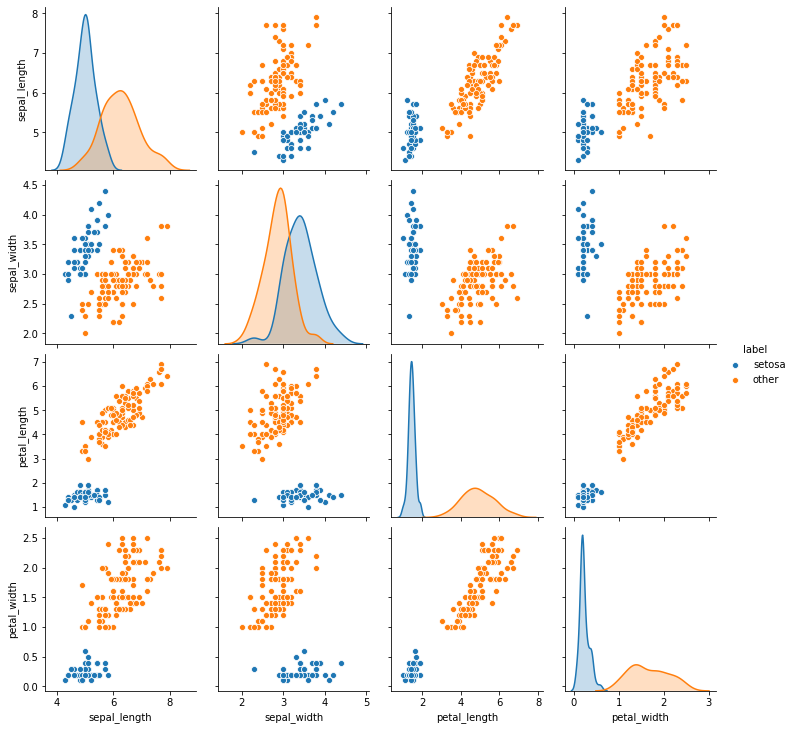
\includegraphics[scale=0.35]{iris_pairs} \\
    \caption{This is an example figure}
    \label{fig:my_label}
\end{figure}

\section{Results and Discussion}
\label{sec4}
For the HMM Hidden State detection, the adjusted closing price data was transformed to daily returns and plotted for an initial inspection in Fig. (1)(a). Fig. (1)(b) shows the two identified hidden states: Hidden State 1 shows a greater variance (5.4e-4) and thus suggests a more volatile market than the one detected in Hidden State 0 (8.5e-5).\\
\\
Figs\\
\\
In the case of an SVM, we see in Fig. (2)(a) that the regimes detected by the algorithm are more refined; Upon first observation, the algorithm detects minor downturns that are not seen in the HMM result, but also includes areas that would be classified as upwards-trending/bull markets by the HMM. This result is mainly dictated by the choice of ν: for a smaller ν, the algorithm generates fewer training errors for each of the support vectors, and could narrow the list of detected regimes by shrinking the margin of classification error (Fig (2)(b) for ν=0.1).\\
\section{Next Steps}
\label{sec5}
The next steps for this project involve the analysis of additional data, such as the VIX index, to illustrate further the existence of hidden states of bull/bear markets in the relevant historical time series. Additionally, the pièce de resistance of any regime detection tool, including the one presented here is their deployment in an actual trading strategy, where the strategy returns would be benchmarked against the market returns to determine their efficacy. The next development of this paper will utilize the regime detection tools and along with a list of market indicators will generate a signal that will track the cumulative returns of a historical time series for a US-exchange listed security. This will ultimately determine whether there is a solid ground for the execution of said trade. Some things to be aware of in the data are autocorrelation of returns and avoiding the pitfall of simply fitting the data to get empirical results that are compatible with the original theoretical postulations.

\subsection*{Acknowledgments}
I would like to thank professor Feinstein for his invaluable guidance through his teachings in FE 690: Machine Learning in Finance, and his continued support in identifying the pain points and potential developments in the project proposal; The Stevens Institute of Technology Department of Financial Engineering for its provision of laptops and technological equipment to undertake this project; and lastly, the unsung heroes that maintain the ambitious Yahoo Finance project at this stage of abandonment from its parent organization.

% Appendix
\appendix
\section{Code}
\label{source_code}
\begin{lstlisting}
Source code (Python Notebook format):

#%%
# Import Packages:
import numpy as np
import pandas as pd
import yfinance as yf
from hmmlearn import hmm
from matplotlib import pyplot as plt
from sklearn.svm import OneClassSVM
from sklearn.preprocessing import PolynomialFeatures

#%%
# SPY also captures volatility well. BBUS too, but there is not enough data. Mainly, they are both US ETFs and are not suitable for the argument I want to make.
# https://www.ishares.com/us/products/239623/ishares-msci-eafe-etf
# is composed of large- and mid-cap developed market equities, excluding the US and Canada.

etf = yf.download('EFA', start='2000-01-01', end='2020-09-24')
print(etf)
etf = etf[['Adj Close', 'Volume']] #Using adjusted close (transformed into daily returns) and volume. What other feature of the set can describe volatility?
print(etf)

#%%
# Initiate HMM instance
hmm_1 = hmm.GaussianHMM(n_components=2, covariance_type="full", n_iter=1000)

#%%
# Transform adjusted close prices to daily returns;
# Remove first adjusted close entry becomes null after the transformation;
# A is our arbitrary Borel set (measurable):
A = np.column_stack([etf['Adj Close'].pct_change()[1:], etf['Volume'][1:]])
print(A[:10])

#%%
# Fit model to set A:
hmm_1.fit(A)

#%%
# Predict states through the HMM instantiation above:
hmm_states = hmm_1.predict(A)
print(hmm_states)
#%%
# Filter states:
hmm_state_0 = hmm_states == 0
hmm_state_1 = hmm_states == 1

#%%
# Extract column for convenience:
close_price = etf['Adj Close'][1:]

#%%
# Plot price data:
default = 'black'
fig = plt.figure(figsize=(25,15))
# Data:
close_price_line = fig.add_subplot(111)
plt.plot_date(close_price.index,close_price, marker='*', ms=5, color='black', alpha=0.3, label='EFA Adj. Close')
# Aesthetic adjustments:
close_price_line.set_title('Adjusted Closing Price, EFA', fontsize=30, color=default)
close_price_line.set_xlabel("Date", fontsize=20, color=default)
close_price_line.set_ylabel("Closing Price", fontsize=20, color=default)
close_price_line.tick_params(axis='both', labelsize=15, colors=default)
close_price_line.legend(loc='upper left', fontsize=15)
# Generate and save graph:
plt.savefig('adj_close_graph.png')
plt.show()

#%%
# Plot states:
default = 'black'
fig = plt.figure(figsize=(25,15))
# Data:
markov_states = fig.add_subplot(111)
plt.plot_date(close_price.index[hmm_state_0],close_price[hmm_state_0], marker='*', ms=5, alpha=0.4, label='Hidden State 0')
plt.plot_date(close_price.index[hmm_state_1],close_price[hmm_state_1], marker='*', ms=5, alpha=0.4, label='Hidden State 1')
# Aesthetic adjustments:
markov_states.set_title('Hidden Markov States', fontsize=30, color=default)
markov_states.set_xlabel("Date", fontsize=20, color=default)
markov_states.set_ylabel("Closing Price", fontsize=20, color=default)
markov_states.tick_params(axis='both', labelsize=15, colors=default)
markov_states.legend(loc='upper left', fontsize=15)
# Generate and save graph:
plt.savefig('hmm_graph.png')
plt.show()
#%%
data = etf['Adj Close'].tolist()
#%%
# Creating monthly partitions/windows that the algorithm uses to predict the current regime.
out = []
for i in range(len(data)):
    train_window = np.array(data[i - 30:i])
    try:
        out.append(train_window / train_window[0])
    except:
        out.append(np.ones(30))

#%%
A = np.array(out)
print(A)

#%%
# Using the Radial Basis Function kernel with default nu value
svm_1 = OneClassSVM(kernel='rbf', gamma=1.0)

#%%
svm_1.fit(PolynomialFeatures(degree=3).fit_transform(A))
print(svm_1)
hmm_states = svm_1.predict(PolynomialFeatures(degree=3).fit_transform(A))
hmm_states_rw = pd.Series(hmm_states).rolling(window=10).mean().fillna(1)
print(hmm_states_rw)

#%%
# Filter HSVM states:
hmm_states_rw[hmm_states_rw >= 0] = 1
hmm_states_rw[hmm_states_rw < 0] = 0
hmm_states = hmm_states_rw
hmm_states.index = etf.index
hmm_state_0_cluster = hmm_states == 0
hmm_state_1_cluster = hmm_states == 1

#%%
# Plot Hidden SVM states:
default = 'black'
fig = plt.figure(figsize=(25,15))
# Data:
hidden_svm_states = fig.add_subplot(111)
plt.plot_date(etf.index[hmm_state_0_cluster],etf['Adj Close'][hmm_state_0_cluster], marker='*', ms=5, alpha=0.4, label='Cluster 0')
plt.plot_date(etf.index[hmm_state_1_cluster],etf['Adj Close'][hmm_state_1_cluster], marker='*', ms=5, alpha=0.4, label='Cluster 1')
# Aesthetic adjustments:
hidden_svm_states.set_title('HMSVM Clusters', fontsize=30, color=default)
hidden_svm_states.set_xlabel("Date", fontsize=20, color=default)
hidden_svm_states.set_ylabel("Closing Price", fontsize=20, color=default)
hidden_svm_states.tick_params(axis='both', labelsize=15, colors=default)
hidden_svm_states.legend(loc='upper left', fontsize=15)
# Generate and save graph:
plt.savefig('hmm_svm_graph.png')
plt.show()
\end{lstlisting}

\printbibliography
\end{document}